\documentclass{cmn}
\usetikzlibrary{shapes.multipart,decorations.pathreplacing,calligraphy}

\tikzset{
  downwardCurlybrace/.style={
    decoration={calligraphic brace,amplitude=5pt,raise=1mm},
    decorate,
    line width=1.25pt
  },
  upwardCurlybrace/.style={
    downwardCurlybrace,
    decoration={mirror}
  }
}

\newlength\cellWidth
\newlength\cellHeight
\setlength\cellWidth{14mm}
\setlength\cellHeight{10mm}

\begin{document}
  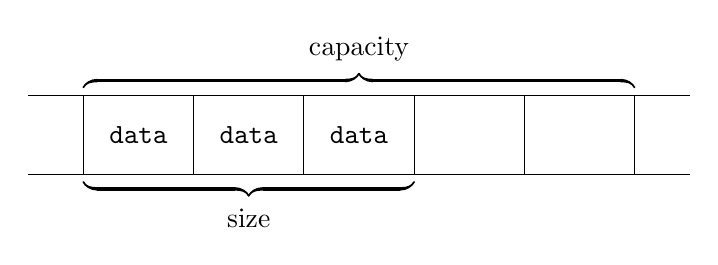
\begin{tikzpicture}
    % borders
    \draw (0,0) -- ++(6*\cellWidth,0);
    \draw (0,-\cellHeight) -- ++(6*\cellWidth,0);

    % cell dividing borders
    \foreach \x in {0,...,5} {
      \pgfmathsetmacro\nx{\x+0.5}
      \draw (\nx*\cellWidth,0) -- ++(0,-\cellHeight);
    }

    % cell text
    \foreach \x in {1,...,3} {
      \node at (\x*\cellWidth,-\cellHeight/2) {\texttt{data}};
    }

    \draw[upwardCurlybrace]
      (\cellWidth/2,-\cellHeight) -- ++(3*\cellWidth,0)
      node[midway, below=3mm] {size};
    \draw[downwardCurlybrace]
      (\cellWidth/2,0) -- ++(5*\cellWidth,0)
      node[midway, above=3mm] {capacity};
  \end{tikzpicture}
\end{document}
